\documentclass{article}

\usepackage{graphicx}
\usepackage[hidelinks]{hyperref}
\usepackage{url} % supplies the \path command we use for a texttt that wraps nicely
\usepackage{booktabs} % \toprule etc
\usepackage[margin=0.6in]{geometry}

\begin{document}

\begin{figure}[h!]
\centering
\centerline{\includegraphics[width=0.64\textwidth]{figures/fig1}}
\caption{\
Nucleotide-level mutation processes distort protein language models, negatively impacting functional predictions.
(\textbf{A}) Distribution of AbLang2 probabilities for amino acids accessible from a naive BCR sequence by single nucleotide mutations versus those requiring multiple mutations from the original codon.
(\textbf{B}) The relationship between neutral somatic hypermutation probability and AbLang2's predicted probability of nonsynonymous mutation for nine different naive sequences. Each point represents a site in the sequence.
Outliers are marked with triangles and brought into the y range.
(\textbf{C}) Correlation between experimental expression measurements and negative pseudo-perplexity predictions from AbLang2, separated by whether variants require single or multiple nucleotide changes.
}%
\label{fig:ntProcessInLLMs}
\end{figure}

\begin{table}[h!]
  \begin{center}
  \begin{tabular}{lccccc}
  & AbLang2 & ESM & ProGen2 & DASM \\
  \midrule
  Koenig G6 Expression & 0.344 & 0.418 & 0.559 & \textbf{0.669} \\
  Koenig G6 Binding & -0.032 & -0.001 & 0.156 & \textbf{0.312} \\
  Shanehsazzadeh 119 Binding & 0.263 & 0.248 & 0.074 & \textbf{0.470} \\
  Shanehsazzadeh 120 Binding & 0.166 & 0.337 & 0.052 & \textbf{0.540} \\
  \bottomrule
  parameters & 45M  & 650M & 151M & \textbf{4M} \\
  execution time (s) & 830 & 6474 & 2990 & \textbf{4.1} \\
  \bottomrule
  \end{tabular}
\end{center}
  \caption{%
  DASMs have substantially better performance for antibody functional prediction yet are smaller and much faster.
  The first four rows show the correlation between prediction and functional data for the largest data sets in the FLAb benchmark repository.
  The last two rows show the number of parameters and the execution time to evaluate 100 sequences on an A100 GPU.
  }
  \label{tab:model-comparison}
\end{table}


\begin{figure}[h!]
\centering
\centerline{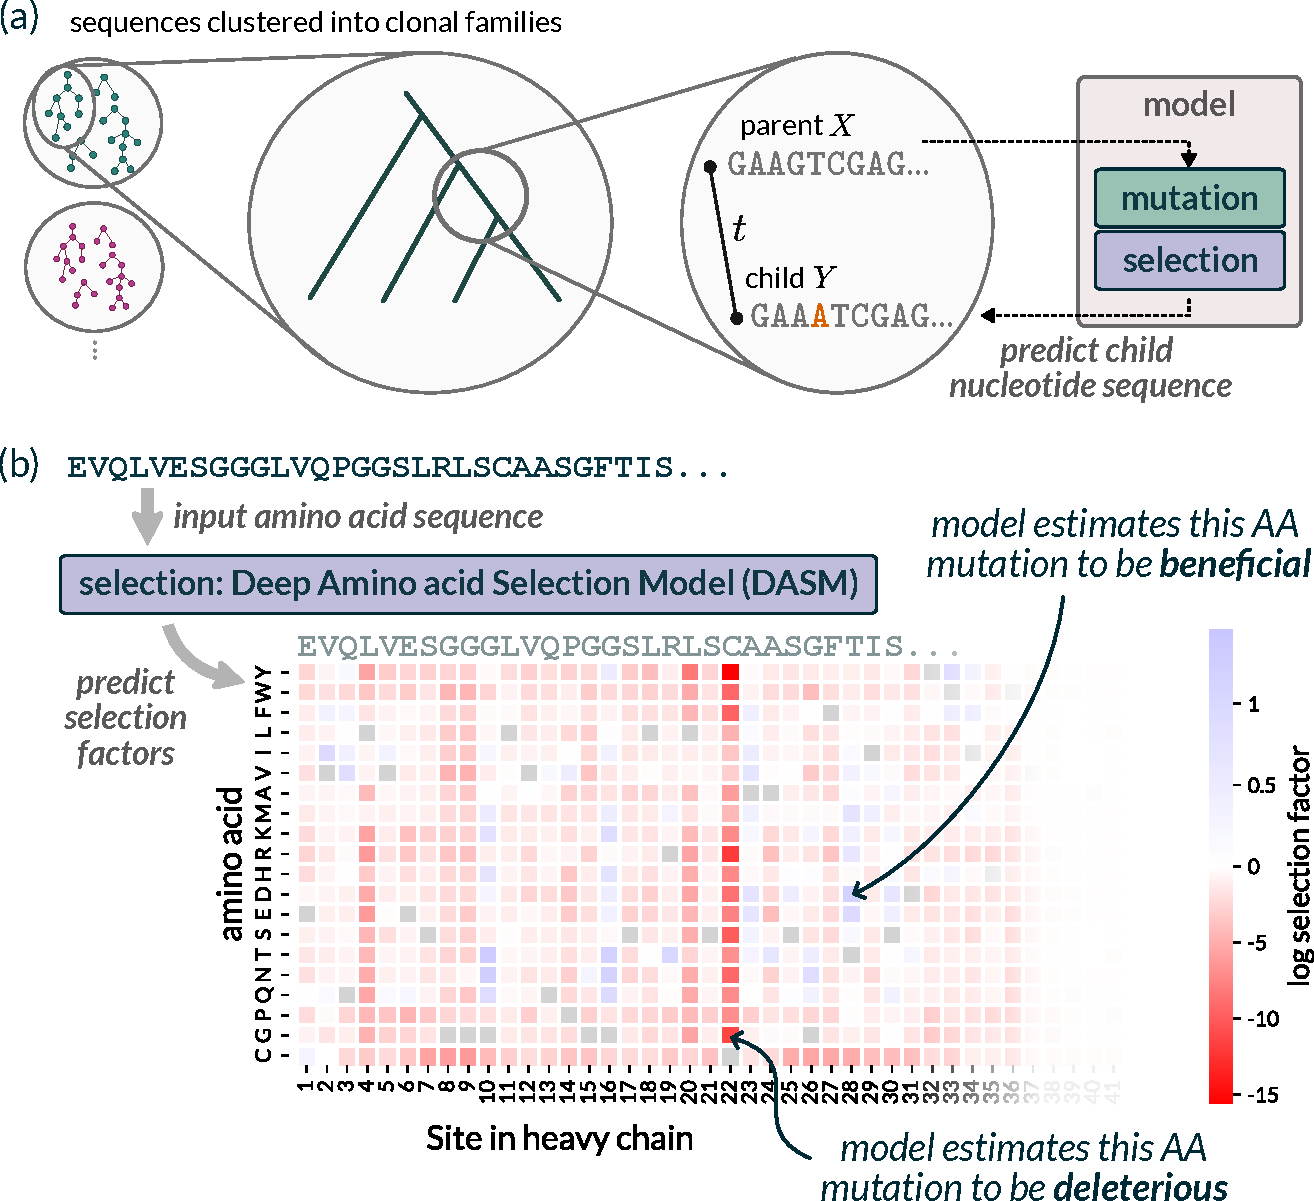
\includegraphics[width=0.9\textwidth]{figures/dasm-output-schematic}}
\caption{\
Our approach separates mutation and selection processes, leading to improved functional prediction and greater interpretability.
(a) The objective of our mutation-selection modeling approach is to predict a child nucleotide sequence given a parent sequence after evolutionary time $t$. 
In the antibody case, the mutation model is a small convolutional neural network trained on separate non-functional data and fixed, while the selection model is a transformer-based Deep Amino Acid Selection Model (DASM). 
This DASM is trained using pairs of parent and child sequences obtained from functional antibody sequences clustered into ``clonal families'', which are collections of sequences that descend from a common ancestor created by VDJ recombination.
The parent-child sequences are then obtained by phylogenetic reconstruction and ancestral sequence inference.
(b) The DASM takes an input amino acid sequence and predicts selection factors for each possible non-wildtype amino acid at every site. 
In terms of molecular evolution, positive values (in log space) indicate that the corresponding amino acid change is more likely than expected under a neutral mutation process. 
Negative values indicate that the amino acid change is less likely than expected. 
Unlike for masked language models, this is done in a single pass with no need for masking.
}%
\label{fig:methods}
\end{figure}


\begin{figure}[ht]
\centering
\centerline{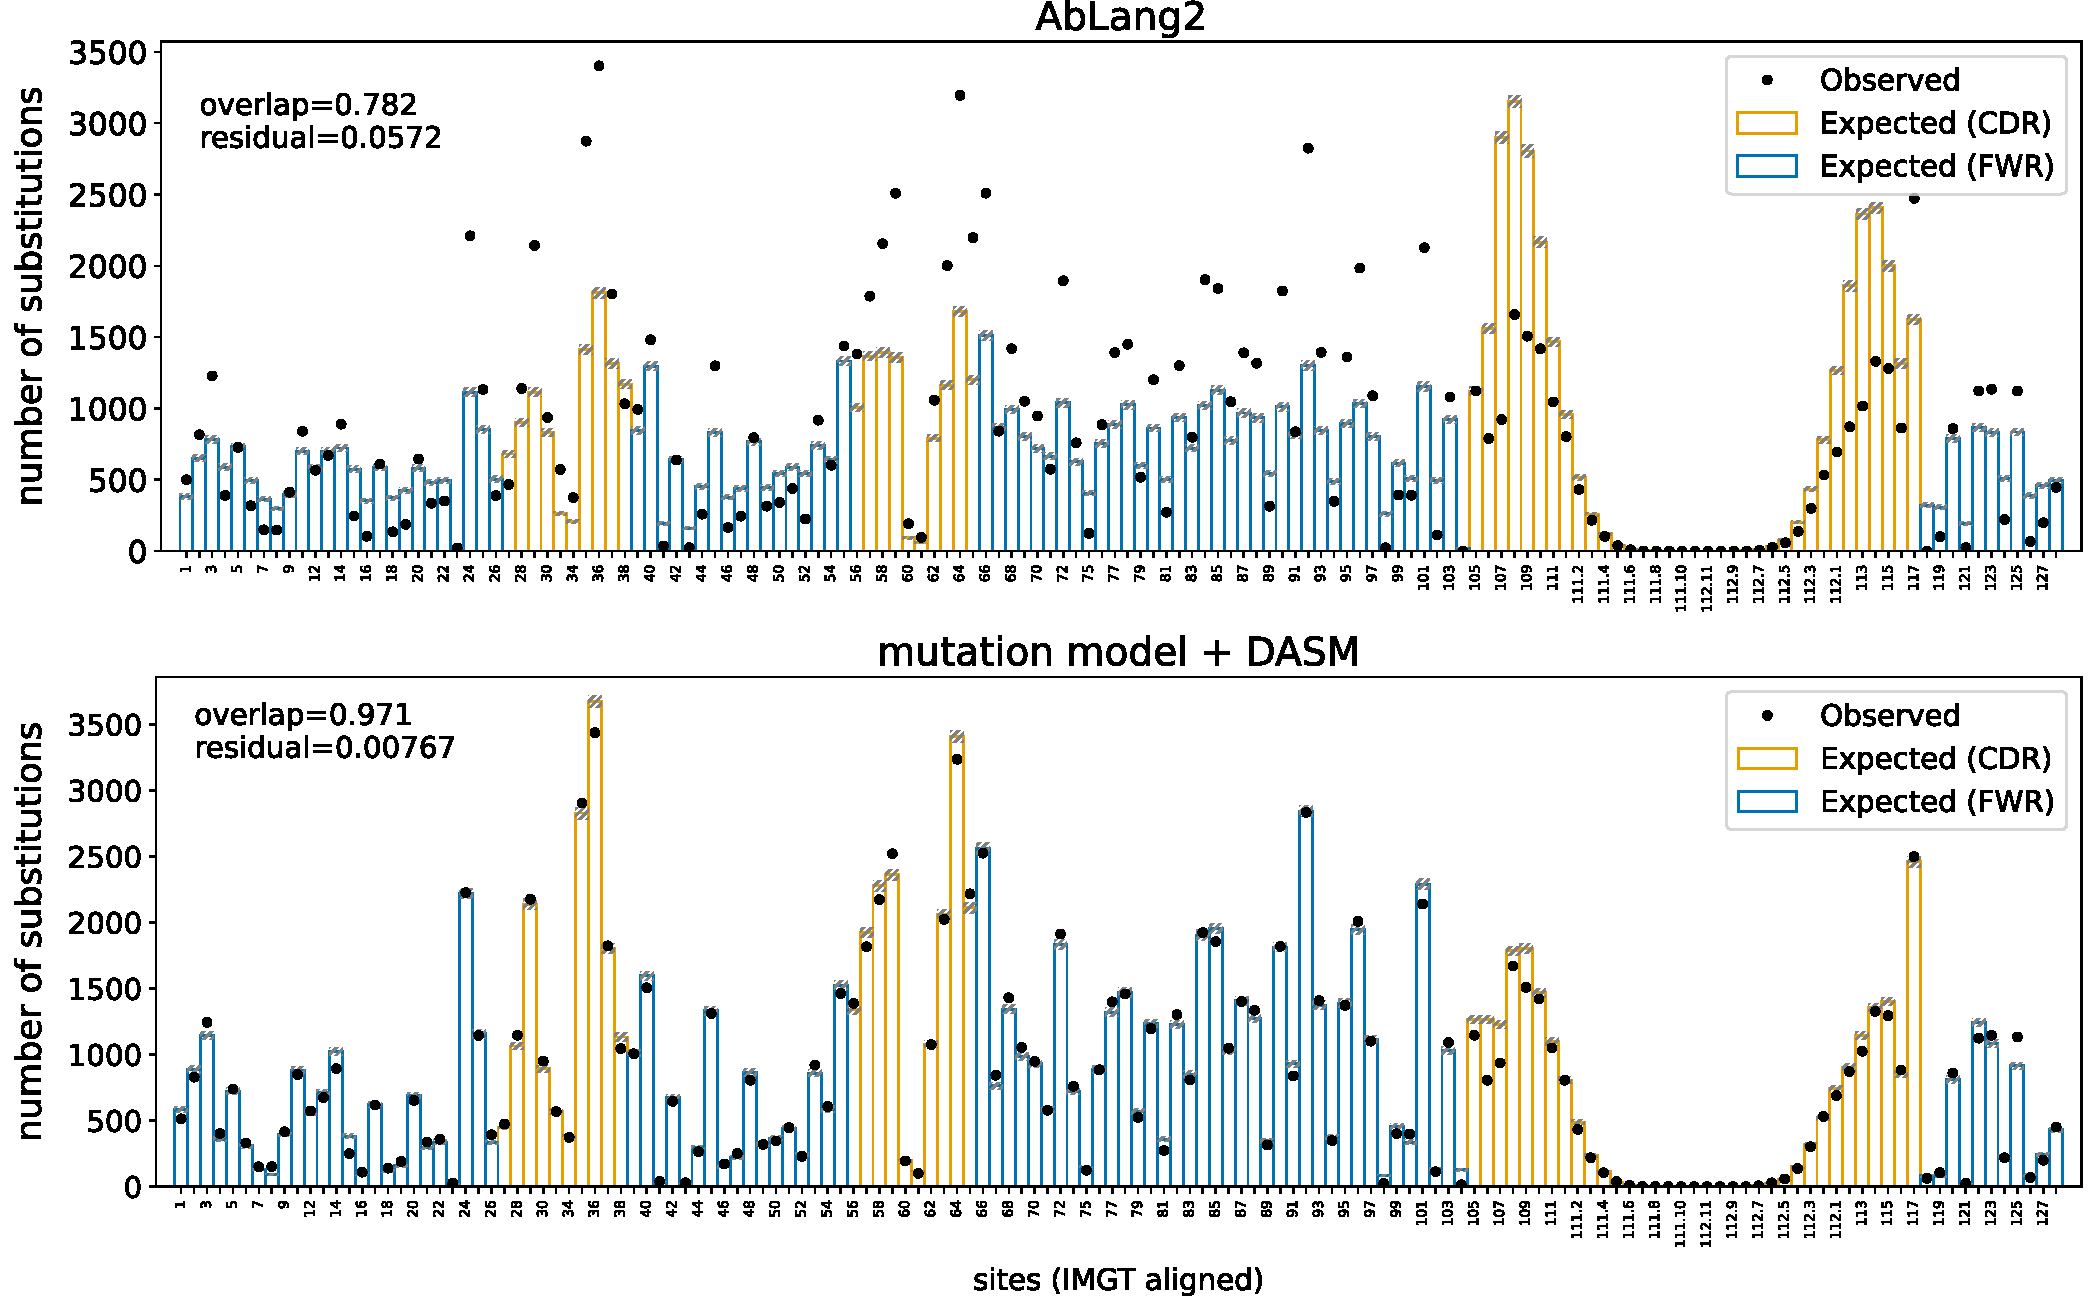
\includegraphics[width=0.75\textwidth]{figures/sites-oe-rodriguez}}
\caption{\
DASMs are much better at predicting child sequences from parent sequences than language models.
Each model was run on a held-out dataset and for each sequence asked to predict the probability that each site would mutate.
The total observed number of mutations is marked with dots, while the total model predictions are shown as a bar plot.
}%
\label{fig:selFactorsAndPerplexity}
\end{figure}


\begin{figure}[h!]
\centering
\centerline{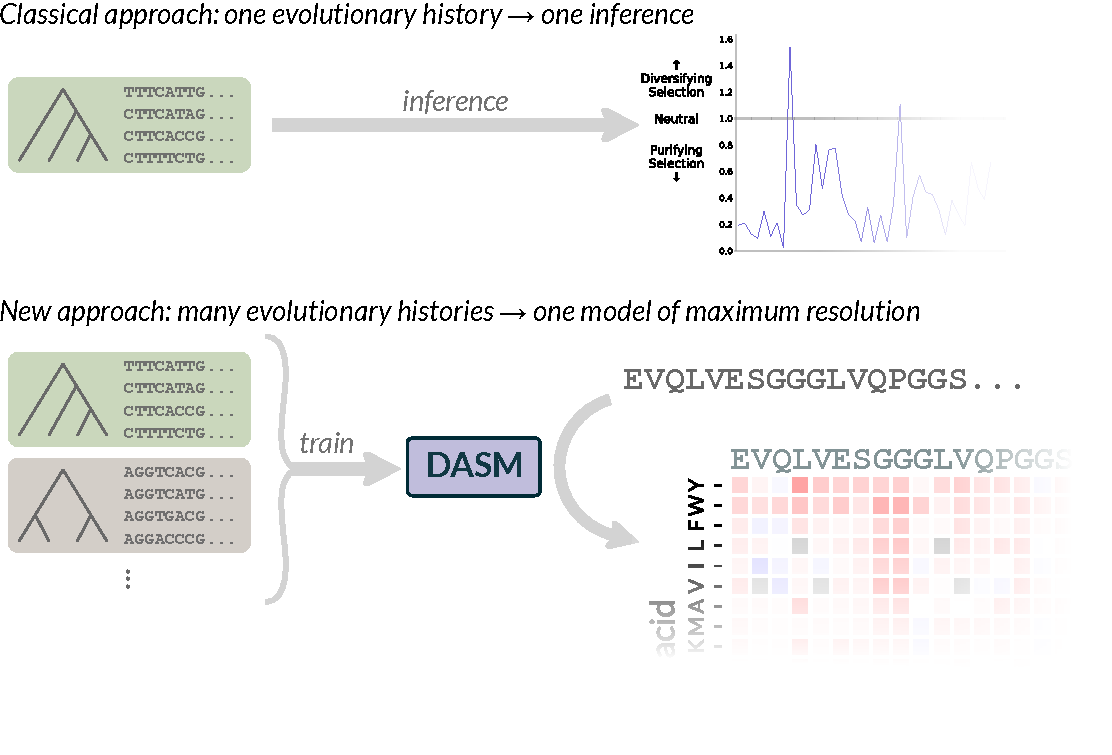
\includegraphics[width=0.9\textwidth]{figures/dasm-paradigm}}
\caption{\
In the classical approach, one performs a single inference for a given sequence alignment. 
In the best-case scenario with lots of data, one can infer a per-site selection factor for that alignment.
In the DASM approach, we train a model on many sequence alignments, and then use that model to predict for any given sequence.
In this way, we are able to use a diversity of sequences to train a model of maximum resolution: per-sequence per-site per-amino-acid.
}%
\label{fig:methods}
\end{figure}




\end{document}